\documentclass[11pt]{ctexart}
\usepackage[margin=2.3cm]{geometry}
\usepackage{graphicx}
\usepackage{siunitx}
\usepackage{booktabs}
\usepackage{amsmath}
\usepackage{amssymb}
\usepackage{xcolor}
\usepackage{caption}
\usepackage{mdframed}
\usepackage[colorlinks=true,linkcolor=blue!60!black,urlcolor=blue!60!black]{hyperref}
\sisetup{detect-all, per-mode=symbol}

\definecolor{good}{HTML}{2E7D46}
\definecolor{bad}{HTML}{B23B3B}
\definecolor{warn}{HTML}{9A6A00}
\newcommand{\cmd}[1]{\texttt{\small #1}}
\captionsetup{font=small}

\title{\bfseries 32\,导 ADS1299 脑电帽\\硬件验收测试方案}
\author{EEG\_MI 项目}
\date{2026 年 7 月 22 日}

\begin{document}
\maketitle

\begin{mdframed}[linecolor=bad,linewidth=1pt,backgroundcolor=bad!5]
\textbf{\textcolor{bad}{关于本文中的图:}} 本文所有插图均为 \textbf{DEMO(合成数据)示例图},由各测试脚本的
\cmd{-{}-demo} 模式生成,仅用于\textbf{展示每个测试跑通后输出的形态与判读方式}。它们\textbf{尚未在真机上采集},
不代表本帽子的真实指标。真机数据需连上帽子后运行对应命令得到。
\end{mdframed}

\begin{abstract}
\noindent
本帽子为 provider DIY 制作,需要在使用前做\textbf{硬件验收}。难点在于:脑电没有绝对标准,不好直接"对答案"。
本方案的核心思路是——\textbf{不依赖"标准脑电",而是用两种可以自己造出来的真值}:\textbf{(1) 电学真值}:给系统注入
\emph{已知}的电压/频率,看它是否如实还原(检验采集链本身);\textbf{(2) 生理真值}:利用几个\emph{极其稳健、人人可复现}
的脑电反应(睁闭眼 $\alpha$、眨眼、咬牙等)作为"生物标定信号"。据此给出一套分层的验收测试,并附每个测试的目的、
方法、判据、命令与示例图。所有测试脚本位于 \cmd{cap32\_acquisition/}(便携文件夹,可整包复制)。
\end{abstract}

\section{验收难点与思路}
DIY 采集系统最常见的问题依次是:\textbf{接线错位}(电极接到错误通道)、\textbf{增益/单位不准}(µV 换算错)、
\textbf{采样时钟不准}(标称 \SI{250}{\hertz} 实际不是)、\textbf{某些通道噪声大/接触差}、\textbf{屏蔽差导致串扰与工频干扰}、
以及 \textbf{WiFi 掉包}。这些都\emph{不需要}脑电标准就能查——要么注入已知信号,要么看系统自身的一致性。最后再用一个
生理测试(睁闭眼 $\alpha$)把\textbf{整条链}一次性验收。

\section{测试总览}
\begin{center}
\small
\begin{tabular}{@{}lllc@{}}
\toprule
类别 & 测试 & 验什么 & 状态 \\
\midrule
电学·本底 & 噪声底 (§\ref{sec:noise}) & 放大器本底噪声 & \textcolor{good}{已建} \\
电学·本底 & 直流/顶轨 (§\ref{sec:dc}) & DC 偏置 \& 饱和 & \textcolor{good}{已建} \\
电学·本底 & 通道串扰 (§\ref{sec:xtalk}) & 布线/屏蔽 & \textcolor{good}{已建} \\
电学·本底 & 工频拾取 (§\ref{sec:mains}) & 抗干扰(CMRR 代理) & \textcolor{good}{已建} \\
注入验证 & 阻抗注入 A/B/A (§\ref{sec:inj}) & 阻抗模式是否真实存在 & \textcolor{good}{已建} \\
生理·标准 & 睁闭眼 $\alpha$ (§\ref{sec:alpha}) & \textbf{整条链}(电极→放大→参考→montage) & \textcolor{good}{已建} \\
\midrule
电学·注入 & 增益准确度 (§\ref{sec:todo}) & µV 换算是否正确 & \textcolor{warn}{待建·需信号源} \\
电学·注入 & 采样率/频率准确度 (§\ref{sec:todo}) & 采样时钟 & \textcolor{warn}{待建·需信号源} \\
电学·注入 & 频响/带宽、线性度 (§\ref{sec:todo}) & 滤波、失真 & \textcolor{warn}{待建·需信号源} \\
接线 & 通道映射核对 (§\ref{sec:todo}) & \textbf{接线是否接反}(DIY 头号风险) & \textcolor{warn}{待建·零设备} \\
系统 & 长时稳定/掉包 (§\ref{sec:todo}) & WiFi 可靠性 & \textcolor{warn}{待建·零设备} \\
生理 & 眨眼/咬牙功能核对 (§\ref{sec:todo}) & 额区/颞区电极+极性 & \textcolor{warn}{待建·零设备} \\
\bottomrule
\end{tabular}
\end{center}

\section{电学·本底测试}
统一由 \cmd{hardware\_check.py} 采集\textbf{原始}数据(不做 CAR、不滤波),每项出一张图。

\subsection{噪声底 Noise floor}\label{sec:noise}
\paragraph{目的}放大器\emph{自身}的输入端噪声(不含电极/人体)——最硬的质量指标。
\paragraph{方法/设置}把所有电极\textbf{短接在一起}(或接到 REF/地),最好用锡纸包住,采几十秒。算每通道 \SIrange{1}{45}{\hertz}
的 RMS 与幅度谱密度(ASD, µV/$\sqrt{\text{Hz}}$)。
\paragraph{判据}ADS1299 @gain24 理想约 \SI{1}{\micro\volt} RMS;实测 \SIrange{1}{3}{\micro\volt} 为好,$>\SI{8}{\micro\volt}$
说明该道有问题。\quad\cmd{python hardware\_check.py -{}-test noise}
\begin{figure}[h]\centering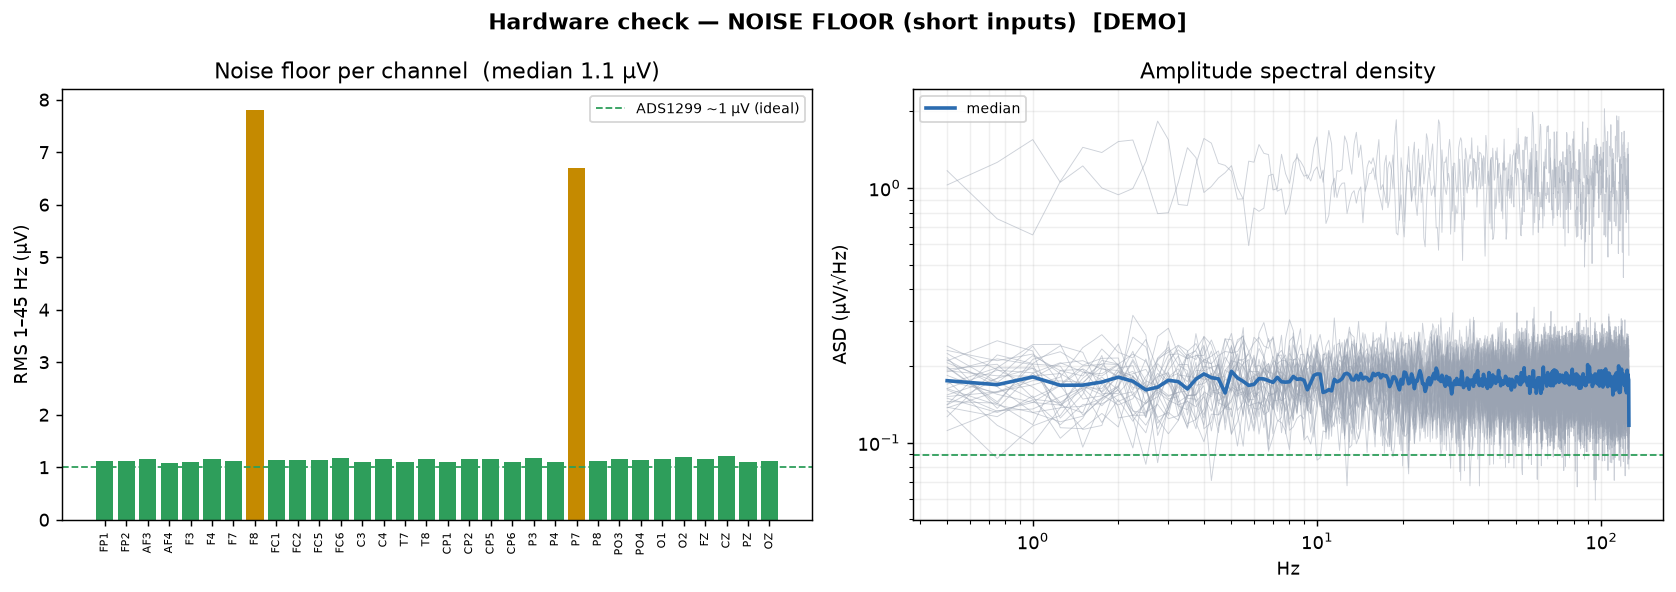
\includegraphics[width=\linewidth]{hw_noise.png}
\caption{\textbf{[DEMO]} 噪声底示例:左为每通道 RMS(绿=好、琥珀=偏高),右为幅度谱密度。合成数据,尚未真机测试。}\end{figure}

\subsection{直流偏置与顶轨 DC offset \& railing}\label{sec:dc}
\paragraph{目的}各通道直流偏置多大、多久顶到 $\pm\SI{187.5}{\milli\volt}$ 满量程(就是把一次录制顶轨的元凶)。
\paragraph{方法/设置}正常戴头上,采原始数据,算每道 DC(mV)与被削顶样本占比。
\paragraph{判据}偏置几十 mV 是干电极极化的\emph{正常}现象;\textbf{顶轨=该道会削顶},需 \SI{1}{\hertz} 高通或重新压电极。
这更多是"干电极+无参考"的问题,\textbf{不一定是板子缺陷}。\quad\cmd{python hardware\_check.py -{}-test dc}
\begin{figure}[h]\centering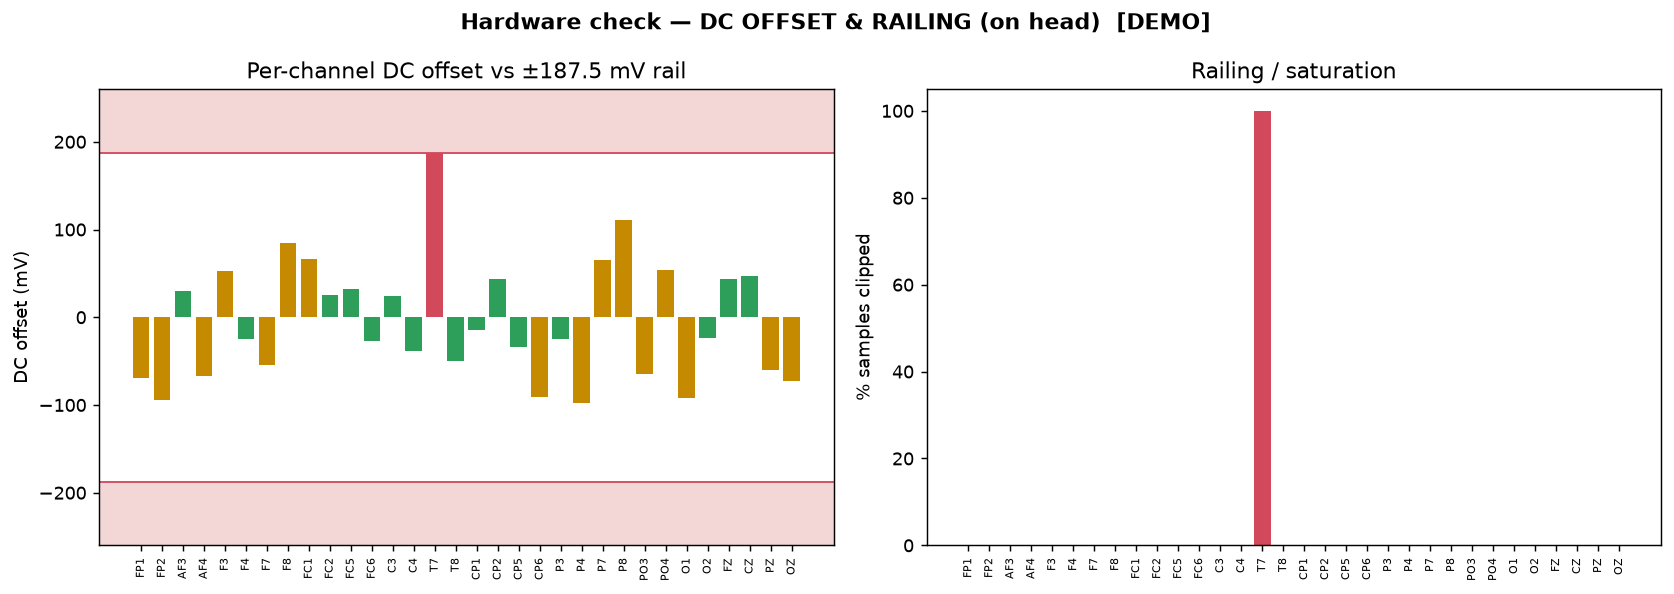
\includegraphics[width=\linewidth]{hw_dc.png}
\caption{\textbf{[DEMO]} DC/顶轨示例:左为各道 DC 偏置对 $\pm\SI{187.5}{\milli\volt}$ 轨(T7 顶轨=红),右为削顶占比。合成数据。}\end{figure}

\subsection{通道串扰 Crosstalk}\label{sec:xtalk}
\paragraph{目的}一个电极上的信号会漏到别的通道多少——直接反映布线/屏蔽,影响 MI 空间分辨。
\paragraph{方法/设置}\textbf{只在一个电极}上加一个干净正弦(信号发生器,或手机播放音调经导线接入),其余不动。
脚本测该频率在其他通道的泄漏比。
\paragraph{判据}$<-\SI{40}{\decibel}$(1\%)= 好隔离;$>-\SI{26}{\decibel}$(5\%)= 布线/屏蔽差。\\
\cmd{python hardware\_check.py -{}-test crosstalk -{}-source-ch C3 -{}-probe-hz 10}
\begin{figure}[h]\centering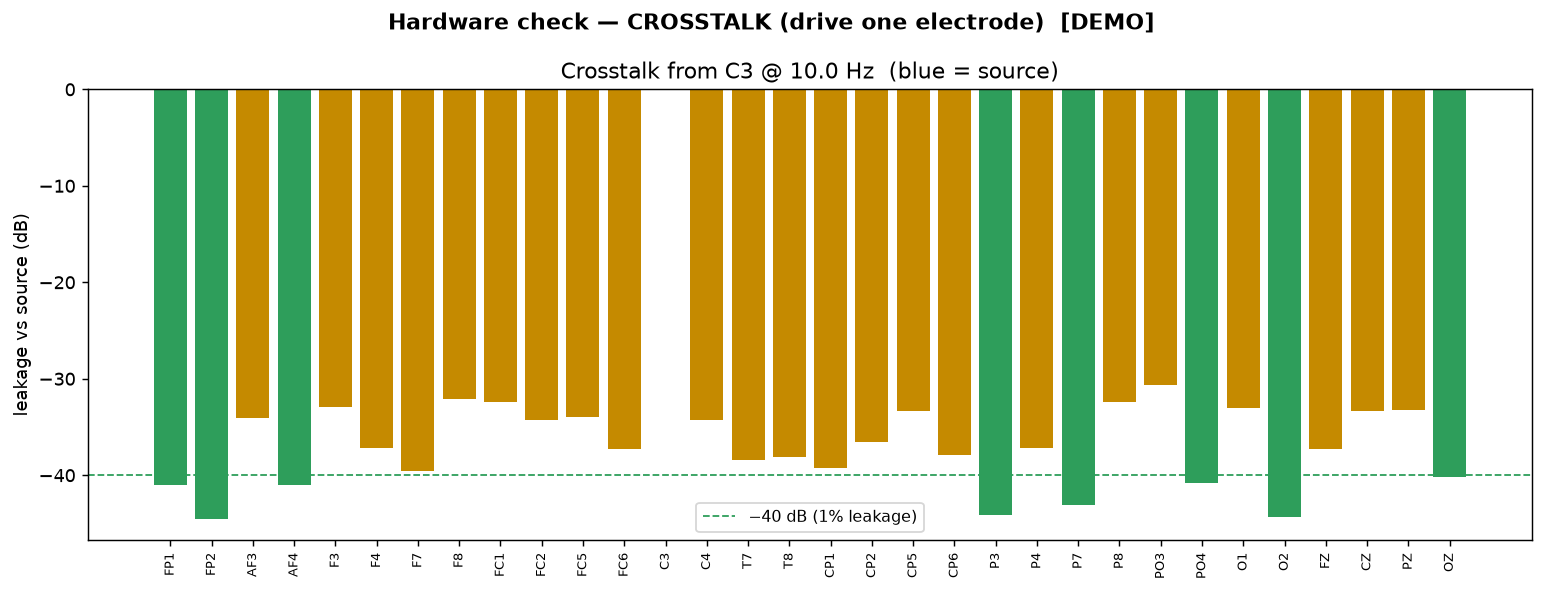
\includegraphics[width=0.86\linewidth]{hw_crosstalk.png}
\caption{\textbf{[DEMO]} 串扰示例:源通道 C3(蓝),其余通道相对源的泄漏(dB),虚线为 $-\SI{40}{\decibel}$。合成数据。}\end{figure}

\subsection{工频拾取 50\,Hz(CMRR 代理)}\label{sec:mains}
\paragraph{目的}各通道拾到多少 \SI{50}{\hertz}——抗干扰能力的实用代理。
\paragraph{方法/设置}正常戴/拿手里,算每道 \SI{50}{\hertz} 幅度及其占总 RMS 比例。
\paragraph{判据}各道\textbf{均匀}的 \SI{50}{\hertz}=共模(CAR+notch 可压);\textbf{个别道特别高}=该道接触/屏蔽差。
真正 CMRR 需"所有输入短接后加共模源",此为实用近似。\quad\cmd{python hardware\_check.py -{}-test mains}
\begin{figure}[h]\centering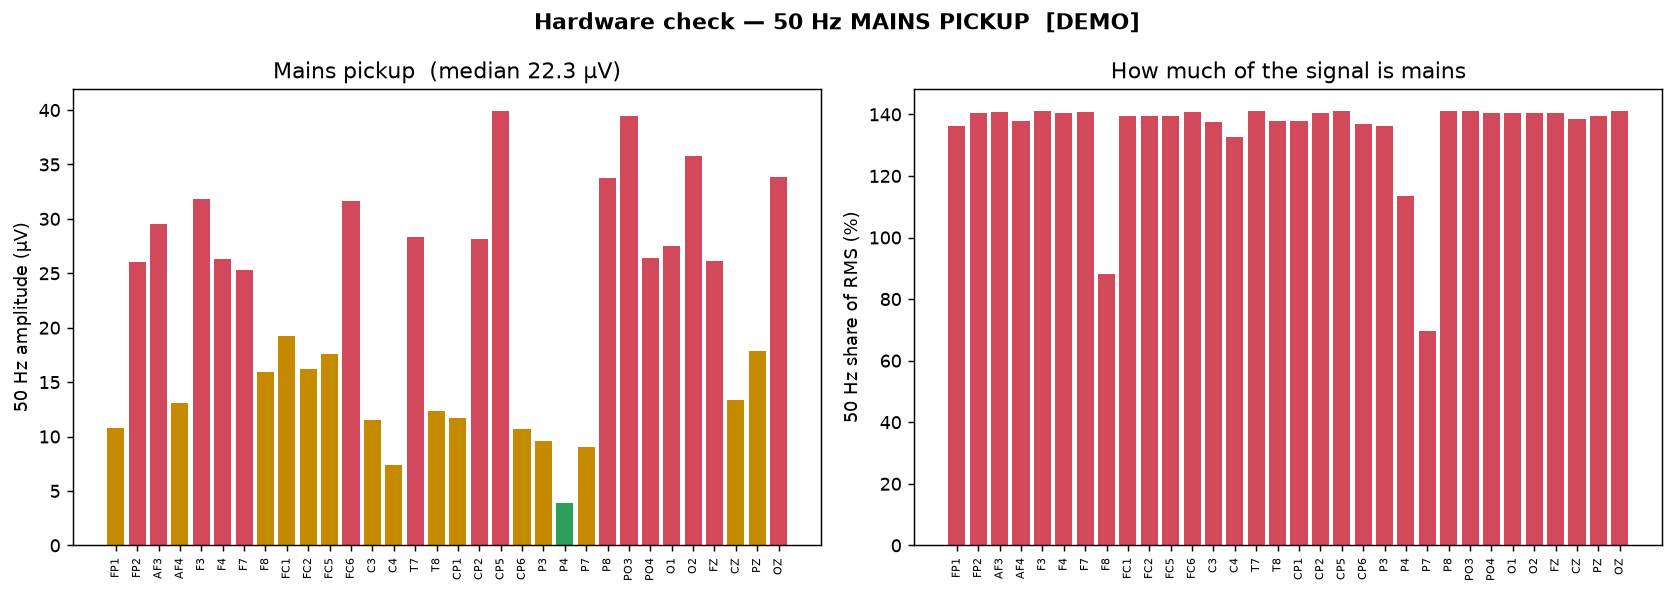
\includegraphics[width=\linewidth]{hw_mains.png}
\caption{\textbf{[DEMO]} 工频示例:左为各道 \SI{50}{\hertz} 幅度,右为其占 RMS 比例。合成数据。}\end{figure}

\section{注入验证:阻抗模式是否真实存在}\label{sec:inj}
\paragraph{目的}验证发送 \texttt{'\%'} 后板子是否真的注入 \SI{31.2}{\hertz} 电流(不是靠推断)。
\paragraph{方法/设置}A/B/A 三段:EEG 模式 $\to$ 阻抗模式 $\to$ EEG 模式;\SI{50}{\hertz} 工频作内置对照。
\paragraph{判据}\SI{31.2}{\hertz} 峰\textbf{仅}在阻抗段出现、遍布所有通道、并随 \texttt{'\%'}/\texttt{'*'} 开关。\quad\cmd{python test\_injection.py -{}-seconds 6}
\begin{figure}[h]\centering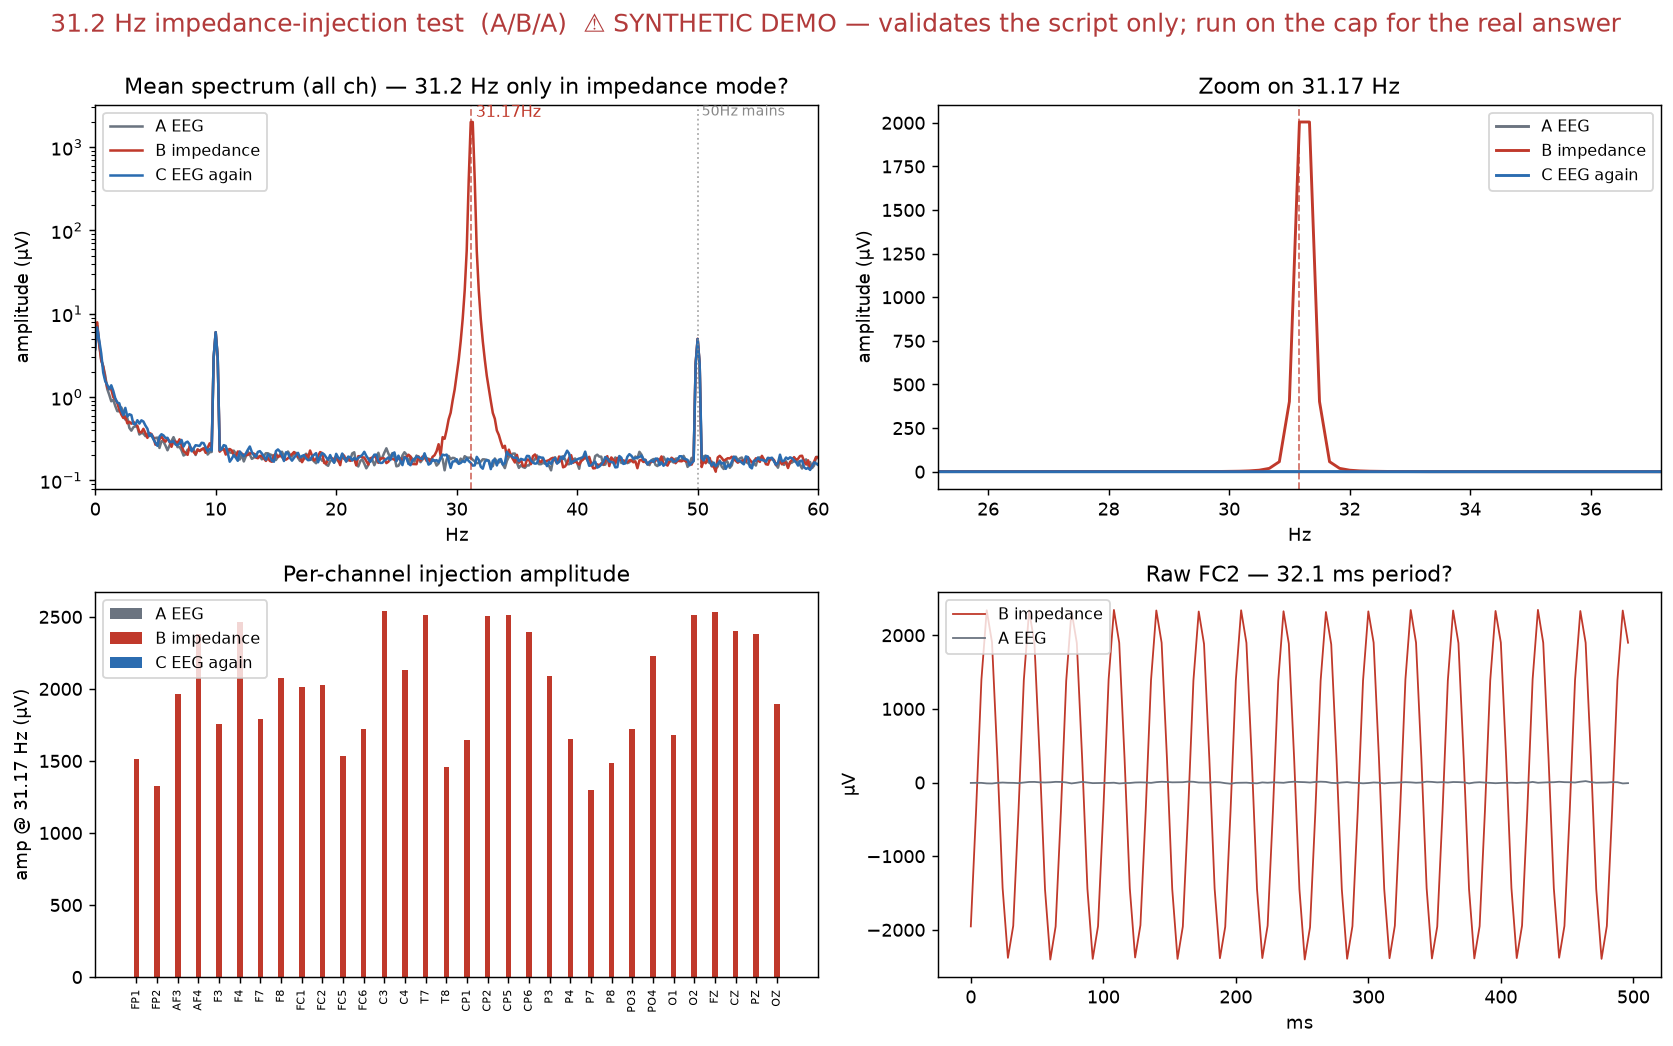
\includegraphics[width=\linewidth]{injection_test_demo.png}
\caption{\textbf{[DEMO]} 注入测试示例(合成)。真机版详见仓库的《阻抗注入实证报告》
(\cmd{impedance\_injection\_report.pdf}),真机实测已确认注入真实存在,且反推电流为\textbf{纳安级($\sim$\SI{24}{\nano\ampere},非微安)};
本图为 demo 合成数据。}\end{figure}

\noindent 配套的 \cmd{impedance\_formula\_check.py} 还会核对厂商两个阻抗换算公式与欧姆定律的矛盾(二者反推的注入电流相差约 $600\times$),
结论是绝对 \si{\kilo\ohm} 不可信,应以相对幅度判断接触。

\section{生理·标准:睁眼/闭眼 $\alpha$(整条链验收)}\label{sec:alpha}
\paragraph{目的}用 Berger 效应作生物标准,一次验收\textbf{整条链}:闭眼 $\to$ 枕区 \SIrange{8}{12}{\hertz} $\alpha$ 暴涨,睁眼 $\to$ 回落。
\textbf{零设备}。若通过,说明电极接触、放大、参考、montage 接线、µV/Hz 量级整体都对。
\paragraph{方法/设置}脚本交替提示睁眼/闭眼各若干段(闭眼放松、别眯眼——眯眼是肌电),比较两态的枕区 $\alpha$ 功率。
\paragraph{判据}\textbf{枕区闭/睁 $\alpha$ 比 $\gtrsim 2\times$ 且以后脑为主}(额区应几乎不变)。\quad\cmd{python alpha\_check.py -{}-blocks 3 -{}-secs 12}
\begin{figure}[h]\centering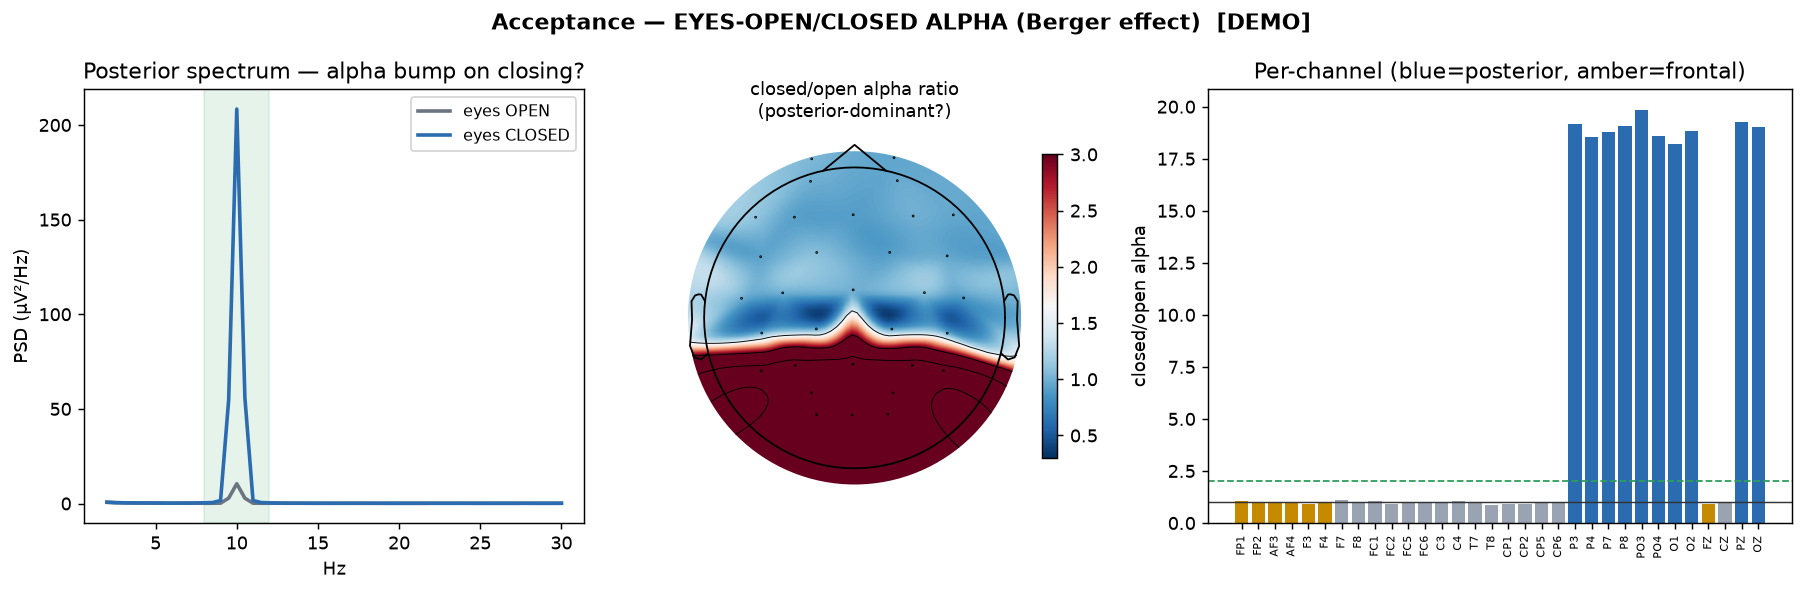
\includegraphics[width=\linewidth]{acceptance_alpha.png}
\caption{\textbf{[DEMO]} 睁闭眼 $\alpha$ 示例:左为枕区谱(闭眼出现 \SI{10}{\hertz} $\alpha$ 峰),中为闭/睁 $\alpha$ 比地形图
(应集中于后脑),右为每通道比值(蓝=枕区、琥珀=额区)。合成数据,尚未真机测试。}\end{figure}

\section{待建测试(建议补齐)}\label{sec:todo}
\paragraph{零设备,可立即安排}
\begin{itemize}
\item \textbf{通道映射/接线核对(头号建议)}:脚本逐个提示,你依次敲/摸一个电极,确认是否点亮\emph{正确通道号}——
查 DIY 最常见的接反/错位。
\item \textbf{长时稳定/掉包}:挂机跑 \SIrange{10}{30}{\minute},用序号计数统计丢包率、有效采样率、断连——WiFi/UDP 可靠性。
\item \textbf{眨眼/咬牙功能核对}:眨眼 $\to$ 额区(FP1/FP2)大偏转;咬牙 $\to$ 颞区(T7/T8)高频暴涨——验额/颞区电极与极性。
\end{itemize}
\paragraph{需要一个信号源(函数发生器,或手机耳机口+分压电阻做 mV 正弦)}
\begin{itemize}
\item \textbf{增益/幅度准确度}:注入已知 mV 正弦,验 µV 换算($\times 0.02235$)是否正确。
\item \textbf{采样率/频率准确度}:注入精确 \SI{10.00}{\hertz},看谱峰落点——验采样时钟。
\item \textbf{频响/带宽 + 混叠、线性度/THD、各道增益一致性}:扫频与逐级加幅度。
\end{itemize}

\section{建议验收顺序}
\begin{enumerate}
\item \textbf{噪声底}(短接输入,现在就能测,最能说明板子本身干不干净);
\item \textbf{通道映射核对}(接反是 DIY 头号风险,务必先排除);
\item \textbf{DC/顶轨、工频}(戴上头);
\item \textbf{睁闭眼 $\alpha$}(整条链一次性验收,零设备);
\item \textbf{阻抗注入 A/B/A}(确认阻抗模式);
\item \textbf{长时稳定/掉包}(挂机);
\item 有信号源后:\textbf{增益、采样率、频响}等注入类精测。
\end{enumerate}

\vspace{0.6em}\noindent\rule{\linewidth}{0.4pt}\\[2pt]
{\small 脚本目录:\cmd{cap32\_acquisition/}(便携整包)。每个测试均带 \cmd{-{}-demo}(合成,无需硬件)用于验证画图。
再次提醒:\textbf{本文所有图为 demo 合成数据示例,尚未真机测试。}}

\end{document}
